\documentclass[11pt]{article}
\usepackage[utf8]{inputenc}
\usepackage{amsfonts}
\usepackage{amsmath}
\usepackage{float}
\usepackage{tikz}
\usetikzlibrary{automata, positioning, arrows}
\tikzset{
  ->,
  >=stealth',
  node distance=3cm,
  every state/.style={thick, fill=gray!10},
  initial text=$ $,
}

\setlength{\parindent}{0em}
\setlength{\parskip}{1em}

\usepackage{geometry}
\geometry{
  a4paper,
  total={170mm,257mm},
  left=20mm,
  top=20mm,
}

\title{Problem Sheet 2}
\author{Rowan Saunders}
\begin{document}

\begin{titlepage}
	\maketitle
\end{titlepage}

\section{Convert NFA to DFA Discussion}
The following is an NFA over the alphabet $\{h,e\}$, for the language:
$$\{w \in \{h,e\}\ast | w \text{ is a repeating pattern of } he \text{ ending in
either } h \text{ or } e \text{ and accepting the empty string}\}$$

\begin{figure}[H]
	\centering
	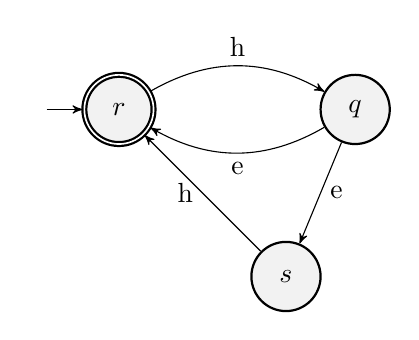
\begin{tikzpicture}
		% states
		\node[state, accepting, initial] (r) {$r$};
		\node[state, right of=r] (q) {$q$};
		\node[state, below right of=r] (s) {$s$};

		% transitions
		\draw (r) edge[bend left, above] node{h} (q)
		(q) edge[bend left, below] node{e} (r)
		(q) edge[right] node{e} (s)
		(s) edge[left] node{h} (r);

	\end{tikzpicture}
	\caption{Laughing NFA}
	\label{fig:laughingnfa}
\end{figure}

ACCEPTS: heh, he, hehehe, heheh

REJECTS: eh, eheh, hheh, heeee

Let $N=(Q,\Sigma,\delta,r,F)$ be a non-deterministic finite automaton, where

\begin{itemize}
	\item $Q = \{r, q, s\}$
	\item $\Sigma = \{h, e\}$
  \item $\delta : Q \times \Sigma_\varepsilon \to \mathcal{P}(Q)$
		\begin{itemize}
			\item $\delta(r,h)=\{q\}$
			\item $\delta(r,e)=\emptyset$
			\item $\delta(q,h)=\emptyset$
			\item $\delta(q,e)=\{r,s\}$
			\item $\delta(s,h)=\{r\}$
			\item $\delta(s,e)=\emptyset$
		\end{itemize}
	\item $r$ is the initial state
	\item $F = \{r\}$
\end{itemize}

\newpage
\subsection{Convert NFA to DFA Discussion, Correction}
The following is an NFA over the alphabet $\{h,e\}$, for the language:
$$\{w \in \{h,e\}\ast | w \text{ is a repeating pattern of } he \text{ ending in
either } h \text{ or } e \text{ and accepting the empty string}\}$$

\begin{figure}[H]
	\centering
	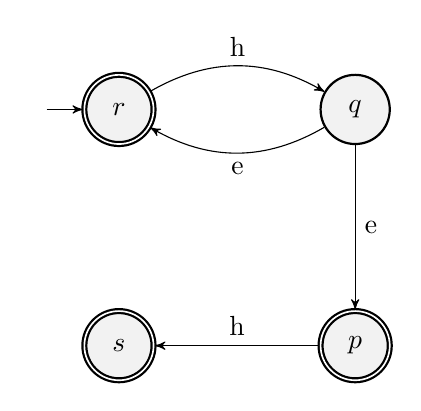
\begin{tikzpicture}
		% states
		\node[state, accepting, initial] (r) {$r$};
		\node[state, right of=r] (q) {$q$};
		\node[state, accepting, below of=r] (s) {$s$};
		\node[state, accepting, below of=q] (p) {$p$};

		% transitions
		\draw (r) edge[bend left, above] node{h} (q)
		(q) edge[bend left, below] node{e} (r)
		(q) edge[right] node{e} (p)
		(p) edge[above] node{h} (s);

	\end{tikzpicture}
	\caption{Laughing NFA}
	\label{fig:laughingnfacorrected}
\end{figure}

ACCEPTS: heh, he, hehehe, heheh, $\varepsilon$

REJECTS: eh, eheh, hheh, heeee, hehheh

Let $N=(Q,\Sigma,\delta,r,F)$ be a non-deterministic finite automaton, where

\begin{itemize}
	\item[] $Q = \{r, q, p, s\}$
	\item[] $\Sigma = \{h, e\}$
	\item[] $\delta : Q \times \Sigma_\varepsilon \to \mathcal{P}(Q)$
		\begin{itemize}
			\item[] $\delta(r,h)=\{q\}$
			\item[] $\delta(r,e)=\emptyset$
			\item[] $\delta(q,h)=\emptyset$
			\item[] $\delta(q,e)=\{r, p\}$
			\item[] $\delta(p,h)=\{s\}$
			\item[] $\delta(p,e)=\emptyset$
			\item[] $\delta(s,h)=\emptyset$
			\item[] $\delta(s,e)=\emptyset$
		\end{itemize}
	\item[] $r$ is the initial state
	\item[] $F = \{r, p, s\}$
\end{itemize}

\subsection{Convert forum post NFA to DFA}
The posted NFA accepts any string from the language $\{0, 1\}$ that starts with
$11$


\begin{figure}[H]
	\centering
	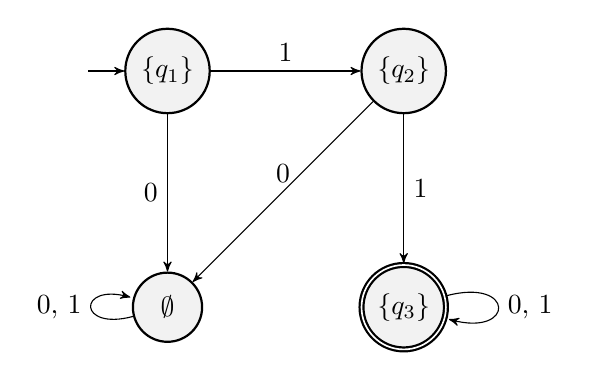
\begin{tikzpicture}
		% states
		\node[state, initial] (q1) {$\{q_1\}$};
		\node[state, right of=q1] (q2) {$\{q_2\}$};
		\node[state, accepting, below of=q2] (q3) {$\{q_3\}$};
		\node[state, below of=q1] (e) {$\emptyset$};

		% transitions
		\draw (q1) edge[above] node{1} (q2)
		(q1) edge[left] node{0} (e)
		(q2) edge[above] node{0} (e)
		(q2) edge[right] node{1} (q3)
		(q3) edge[loop right] node{0, 1} (q3)
		(e) edge[loop left] node{0, 1} (e);

	\end{tikzpicture}
	\caption{Agnes' NFA}
	\label{fig:agnesnfa}
\end{figure}

\newpage
\section{Non-Deterministic Finite Automata Notes}
As before, a (deterministic) finite automata is a 5-tuple $ (Q, \Sigma, \delta,
s_0, F) $ where $Q$ is a finite set of states, $\Sigma$ is the input alphabet,
$\delta : Q \times \Sigma \to Q$ is the transition function, $s_0 \in Q$ is the
start state, $F \subseteq Q$ is the set of accept states.

For a Deterministic Finite Automata (DFA), all valid states must have a
transition function for every member of the input alphabet

For a Non-Deterministic Finite Automata (NFA), the transition function may have
duplicate or missing transitions for members of the input alphabet

Formally, the only difference between an NFA and DFA is the transition function.

For a DFA: $$\delta : Q \times \Sigma \to Q$$

For an NFA we first need to define a mathematical concept called a Power Set

Given a set $A$, the \textbf{power set} of $A$, denoted $\mathcal{P}(A)$, is the
set of all subsets of A.

So, Let $S=\{1,2\}$

$$\mathcal{P}(S)=\{\emptyset,\{1\}, \{2\}, \{1,2\}\}$$

Therefore, for an NFA, the transition function is as follows:

$$\delta : Q \times \Sigma_\varepsilon \to \mathcal{P}(Q)$$

Where $\mathcal{P}(Q)$ is the power set of $Q$, and $\Sigma_\varepsilon = \Sigma
\cup \{\varepsilon\}$ (the alphabet plus the empty string) Therefore, the
transition function returns some set of states from $Q$.

The full formal definition for a Non-Deterministic Finite Automata is a 5-tuple

$$ (Q, \Sigma, \delta, s_0, F) $$

Where $Q$ is a finite set of states, $\Sigma$ is the input alphabet, $\delta : Q
\times \Sigma_\varepsilon \to \mathcal{P}(Q)$ is the transition function, $s_0
\in Q$ is the start state, $F \subseteq Q$ is the set of accept states.

The following diagram is an example NFA

\begin{figure}[H]
	\centering
	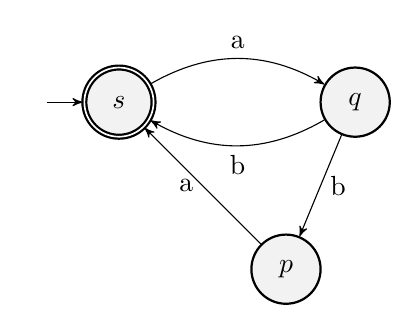
\begin{tikzpicture}
		% states
		\node[state, accepting, initial] (s) {$s$};
		\node[state, right of=s] (q) {$q$};
		\node[state, below right of=s] (p) {$p$};

		% transitions
		\draw (s) edge[bend left, above] node{a} (q)
		(q) edge[bend left, below] node{b} (s)
		(q) edge[right] node{b} (p)
		(p) edge[left] node{a} (s);

	\end{tikzpicture}
	\caption{NFA Example}
	\label{fig:nfaexample}
\end{figure}


For the FSM in \emph{Figure \ref{fig:nfaexample}}:

Let $N=(Q,\Sigma,\delta,s,F)$ be a non-deterministic finite automaton, where

\begin{itemize}
	\item $Q = \{p, q, s\}$
	\item $\Sigma = \{a, b\}$
  \item $\delta : Q \times \Sigma_\varepsilon \to \mathcal{P}(Q)$
		\begin{itemize}
			\item $\delta(s,a)=\{q\}$
			\item $\delta(s,b)=\emptyset$
			\item $\delta(p,a)=\{s\}$
			\item $\delta(p,b)=\emptyset$
			\item $\delta(q,a)=\emptyset$
			\item $\delta(q,b)=\{s,p\}$
		\end{itemize}
	\item $s$ is the initial state
	\item $F = \{s\}$
\end{itemize}

The empty set ($\emptyset$) in the transition function is used to show that
those inputs have no combination of state and symbol/arrow, and result in
immediate rejection.

The definition of a configuration remains the same for an NFA as it was for a
DFA, namely:
\begin{quote}
The combination of a state and a string is a configuration.
A configuration is a pair: $(q, w) \in Q \times \Sigma\ast, (q \in Q, w \in
	\Sigma\ast)$.
\end{quote}

However, the definition of computation for a DFA must be an updated for an NFA

For a DFA the following represents a computation:
\begin{quote}
Let $(q, w)$ and $(q', w')$ be configurations, where:
$$w = aw'$$
for some letter $a \in \Sigma$, and
$$\delta(q, a) = q'$$
Then we say that $(q, w)$ yields $(q', w')$ in one step.

For configurations $(q, w)$ and $(q', w')$ we say that $(q, w)$ yields $(q', w'$
if there is a finite sequence of configurations
$$(q_1, w_1), (q_2, w_2), ..., (q_k, w_k)$$
Such that $(q_1, w_1)=(q,w), (q_k, w_k)=(q',w')$, and
$(q_i, w_i)$ yields $(q_{i+1}, w_{i+1})$ in one step for all $i=1, 2, ..., k-1$
\end{quote}

For an NFA, we replace the definition of "yield in one step" from
$\delta(q,a)=q'$ to $\delta(q,a) \ni q'$, such that the new state goes from
being equal to the result of the transition function, to being a member of the
set of possible states returned from the transition function. Note that a
backwards version of the set membership symbol is used purely for symmetry with
the old version. This could be written as $q' \in \delta(q,a)$. Additionally, we
also need to allow the letter to be include the empty string, by using
$\Sigma_\varepsilon$

So, the full definition for an NFA is:

Let $(q, w)$ and $(q', w')$ be configurations, where:
$$w = aw'$$
for some letter $a \in \Sigma_\varepsilon$, and
$$\delta(q, a) \ni q'$$
Then we say that $(q, w)$ yields $(q', w')$ in one step.

For configurations $(q, w)$ and $(q', w')$ we say that $(q, w)$ yields $(q', w'$
if there is a finite sequence of configurations
$$(q_1, w_1), (q_2, w_2), ..., (q_k, w_k)$$
Such that $(q_1, w_1)=(q,w), (q_k, w_k)=(q',w')$, and
$(q_i, w_i)$ yields $(q_{i+1}, w_{i+1})$ in one step for all $i=1, 2, ..., k-1$

The sequence of configurations defined above for an NFA is called a \textbf{computation}
 
The non-deterministic finite automaton $N=(Q, \Sigma, \delta, s_0, F)$
\textbf{accepts} the string $w \in \Sigma\ast$ if $(s_0, w)$ yields $(q,
\varepsilon)$ where $q \in F$.

Recalling the following definitions:
\begin{quote}
We say that the finite automaton $M$ \textbf{recognises} the language $A$ if
$A=\{w|M \quad \mathrm{accepts} \quad w\}$.

The language \textbf{recognised by} a finite automaton $M$ is denoted $L(M)$.

The language $A$ is called regular if there exists some finite automaton $M$
such that $A = L(M)$. (i.e. a finite automaton exists that recognises it)
\end{quote}

Two finite automata $A$ and $B$ (deterministic or non-deterministic) over the same
alphabet $\Sigma$ are called \textbf{equivalent} if $L(A)=L(B)$, i.e. they
accept the same language.

The above definition leads to the following Theorem:
\begin{quote}
	For every non-deterministic finite automaton $A$ there exists a deterministic
	finite automaton $A'$ which is equivalent to $A$.
\end{quote}

This Theorem has the following proof:
\begin{quote}
	Let $N=(Q,\Sigma,\delta,s_0,F)$ be some non-deterministic finite automaton. We
	construct a deterministic finite automaton $M=(Q',\Sigma,\delta',s_0',F')$
	such that $L(N) = L(M)$.

	Let $Q'=\mathcal{P}(Q)$

	Let $s_0' = E(\{s_0\})$,
	where $E(R)= \{q|q$ is reachable from $R$ by $\varepsilon$ transitions$\}$

	Let $F'=\{R \in Q'|R$ contains an accept state of $N\}$, Alternatively $F'=\{R
	\in Q'|R \cap F \neq \emptyset\}$

	For $R \in Q', a \in \Sigma$, Let $\delta'(R,a)=\{q|q \in E(\delta(r,a)) \quad
	\mathrm{for some} \quad r \in R\}$

	Notice $\delta'(R,a) \in Q'$
\end{quote}

\end{document}
